% Figura: fluxograma do AisleBased
\documentclass[tikz,border=4pt]{standalone}
\usepackage[utf8]{inputenc}
\usepackage[T1]{fontenc}
\usepackage{helvet}
\renewcommand{\familydefault}{\sfdefault}
\usepackage{amsmath}
\usepackage[eulergreek]{sansmath}
\sansmath
\usetikzlibrary{shapes.geometric,arrows.meta,positioning,fit,backgrounds,calc}
\tikzset{
  etapa/.style={draw=blue!60!black, rounded corners=4pt, fill=blue!4, inner sep=8pt},
  bloco/.style={draw=black!70, rounded corners=2pt, fill=white, align=center,
                font=\small, minimum height=1.1cm, text width=2.9cm},
  decisao/.style={diamond, draw=black!70, fill=yellow!15, aspect=1.8, align=center,
                  font=\small, inner sep=1pt},
  fim/.style={draw=black!70, rounded corners=8pt, fill=green!12, align=center,
              font=\small, minimum height=1.0cm, text width=3.1cm},
  falha/.style={draw=red!60!black, rounded corners=8pt, fill=red!8, align=center,
                font=\small, minimum height=0.8cm},
  seta/.style={-{Stealth[length=2.2mm]}, line width=0.7pt},
  rotetapa/.style={font=\small\bfseries, text=blue!60!black, anchor=south west},
}
\begin{document}
\hyphenpenalty=10000\exhyphenpenalty=10000
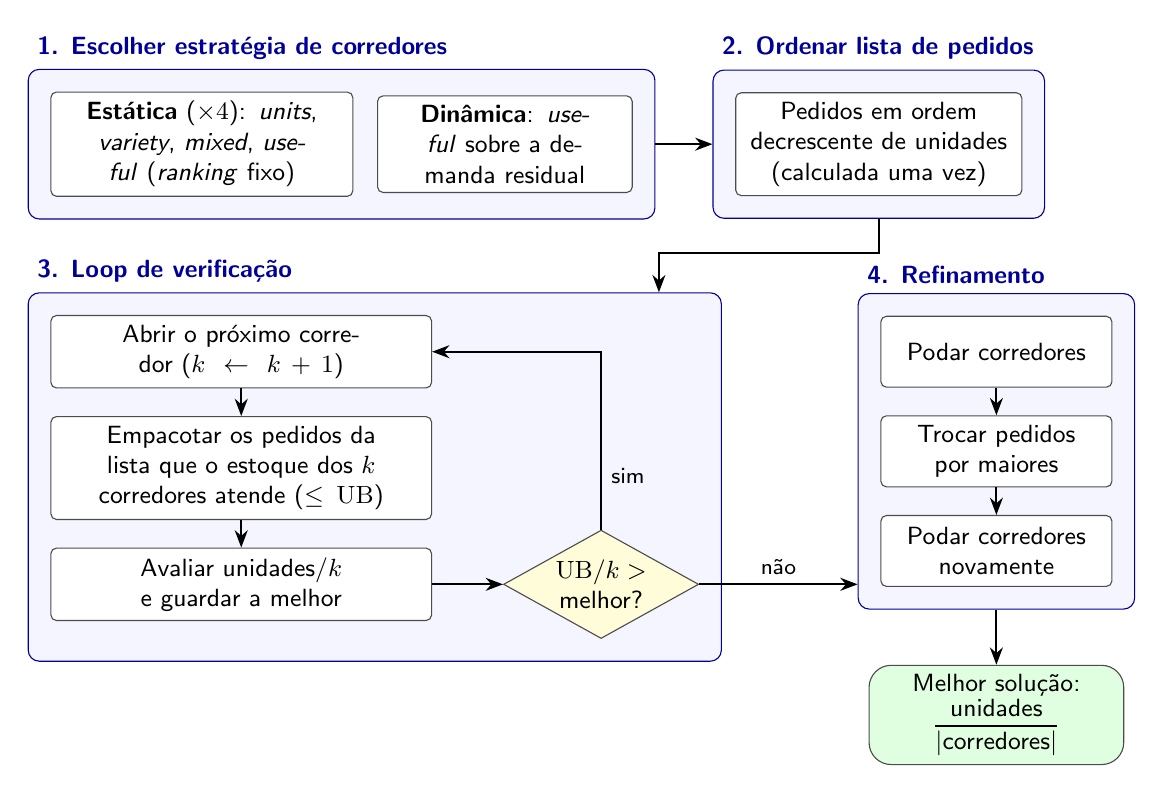
\begin{tikzpicture}[node distance=0.35cm]
\tikzset{pq/.style={bloco, minimum height=0.9cm}}

% ---------- 1. Escolher estratégia de corredores ----------
\node[pq, text width=3.6cm] (est) {\textbf{Estática} ($\times 4$): \textit{units}, \textit{variety}, \textit{mixed}, \textit{useful} (\textit{ranking} fixo)};
\node[pq, right=0.3cm of est, text width=3.0cm] (din) {\textbf{Dinâmica}: \textit{useful} sobre a demanda residual};
\begin{scope}[on background layer]
  \node[etapa, fit=(est)(din)] (e1) {};
\end{scope}
\node[rotetapa] at (e1.north west) {1. Escolher estratégia de corredores};

% ---------- 2. Ordenar lista de pedidos ----------
\node[pq, right=1.3cm of din, text width=3.4cm] (ord) {Pedidos em ordem decrescente de unidades (calculada uma vez)};
\begin{scope}[on background layer]
  \node[etapa, fit=(ord)] (e2) {};
\end{scope}
\node[rotetapa] at (e2.north west) {2. Ordenar lista de pedidos};
\draw[seta] (e1) -- (e2);

% ---------- 3. Loop de verificação ----------
\node[pq, below=1.5cm of est.south west, anchor=north west, text width=4.6cm] (abre) {Abrir o próximo corredor ($k \gets k+1$)};
\node[pq, below=of abre, text width=4.6cm] (emp) {Empacotar os pedidos da lista que o estoque dos $k$ corredores atende ($\leq \mathrm{UB}$)};
\node[pq, below=of emp, text width=4.6cm] (aval) {Avaliar $\text{unidades}/k$ e guardar a melhor};
\node[decisao, right=0.9cm of aval] (pare) {$\mathrm{UB}/k >$\\melhor?};
\begin{scope}[on background layer]
  \node[etapa, fit=(abre)(emp)(aval)(pare)] (e3) {};
\end{scope}
\node[rotetapa] at (e3.north west) {3. Loop de verificação};
\draw[seta] (abre) -- (emp);
\draw[seta] (emp) -- (aval);
\draw[seta] (aval) -- (pare);
\draw[seta] (pare.north) -- node[right, font=\footnotesize, pos=0.3] {sim} (pare.north |- abre.east) -- (abre.east);
\draw[seta] (e2.south) |- ($(e3.north east)+(0,0.5)$) -| ([xshift=-0.8cm]e3.north east);

% ---------- 4. Refinamento ----------
\node[pq, right=2.3cm of pare.east |- abre, text width=2.7cm] (pod1) {Podar corredores};
\node[pq, below=of pod1, text width=2.7cm] (troca) {Trocar pedidos por maiores};
\node[pq, below=of troca, text width=2.7cm] (pod2) {Podar corredores novamente};
\begin{scope}[on background layer]
  \node[etapa, fit=(pod1)(troca)(pod2)] (e4) {};
\end{scope}
\node[rotetapa] at (e4.north west) {4. Refinamento};
\draw[seta] (pod1) -- (troca);
\draw[seta] (troca) -- (pod2);
\draw[seta] (pare.east) -- node[above, font=\footnotesize] {não} (pare.east -| e4.west);

\node[fim, below=0.7cm of e4, text width=3.0cm] (res) {Melhor solução:\\$\dfrac{\text{unidades}}{|\text{corredores}|}$};
\draw[seta] (e4) -- (res);

\end{tikzpicture}
\end{document}
